% Created by tikzDevice version 0.10.1 on 2016-08-15 15:23:26
% !TEX encoding = UTF-8 Unicode
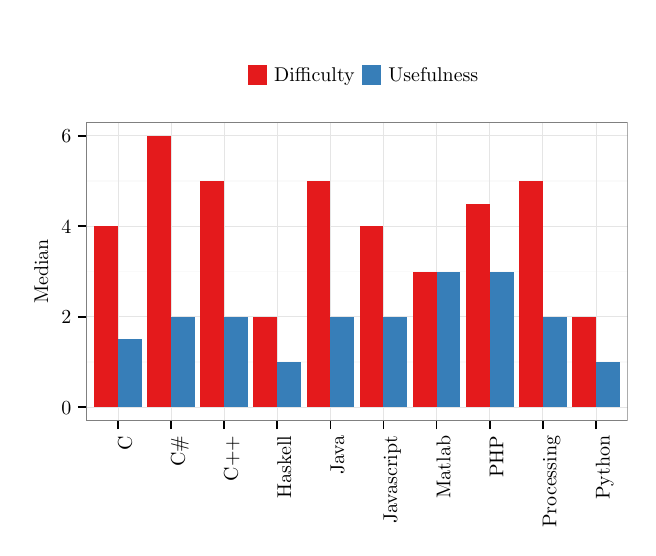
\begin{tikzpicture}[x=1pt,y=1pt]
\definecolor{fillColor}{RGB}{255,255,255}
\path[use as bounding box,fill=fillColor,fill opacity=0.00] (0,0) rectangle (216.81,180.67);
\begin{scope}
\path[clip] (  0.00,  0.00) rectangle (216.81,180.67);
\definecolor{drawColor}{RGB}{255,255,255}
\definecolor{fillColor}{RGB}{255,255,255}

\path[draw=drawColor,line width= 0.6pt,line join=round,line cap=round,fill=fillColor] ( -0.00,  0.00) rectangle (216.81,180.68);
\end{scope}
\begin{scope}
\path[clip] ( 21.16, 38.59) rectangle (216.81,146.53);
\definecolor{fillColor}{RGB}{255,255,255}

\path[fill=fillColor] ( 21.16, 38.59) rectangle (216.81,146.53);
\definecolor{drawColor}{gray}{0.98}

\path[draw=drawColor,line width= 0.6pt,line join=round] ( 21.16, 59.85) --
	(216.81, 59.85);

\path[draw=drawColor,line width= 0.6pt,line join=round] ( 21.16, 92.56) --
	(216.81, 92.56);

\path[draw=drawColor,line width= 0.6pt,line join=round] ( 21.16,125.27) --
	(216.81,125.27);
\definecolor{drawColor}{gray}{0.90}

\path[draw=drawColor,line width= 0.2pt,line join=round] ( 21.16, 43.50) --
	(216.81, 43.50);

\path[draw=drawColor,line width= 0.2pt,line join=round] ( 21.16, 76.21) --
	(216.81, 76.21);

\path[draw=drawColor,line width= 0.2pt,line join=round] ( 21.16,108.92) --
	(216.81,108.92);

\path[draw=drawColor,line width= 0.2pt,line join=round] ( 21.16,141.63) --
	(216.81,141.63);

\path[draw=drawColor,line width= 0.2pt,line join=round] ( 32.67, 38.59) --
	( 32.67,146.53);

\path[draw=drawColor,line width= 0.2pt,line join=round] ( 51.85, 38.59) --
	( 51.85,146.53);

\path[draw=drawColor,line width= 0.2pt,line join=round] ( 71.03, 38.59) --
	( 71.03,146.53);

\path[draw=drawColor,line width= 0.2pt,line join=round] ( 90.21, 38.59) --
	( 90.21,146.53);

\path[draw=drawColor,line width= 0.2pt,line join=round] (109.39, 38.59) --
	(109.39,146.53);

\path[draw=drawColor,line width= 0.2pt,line join=round] (128.57, 38.59) --
	(128.57,146.53);

\path[draw=drawColor,line width= 0.2pt,line join=round] (147.76, 38.59) --
	(147.76,146.53);

\path[draw=drawColor,line width= 0.2pt,line join=round] (166.94, 38.59) --
	(166.94,146.53);

\path[draw=drawColor,line width= 0.2pt,line join=round] (186.12, 38.59) --
	(186.12,146.53);

\path[draw=drawColor,line width= 0.2pt,line join=round] (205.30, 38.59) --
	(205.30,146.53);
\definecolor{fillColor}{RGB}{55,126,184}

\path[fill=fillColor] ( 32.67, 43.50) rectangle ( 41.30, 68.03);
\definecolor{fillColor}{RGB}{228,26,28}

\path[fill=fillColor] ( 24.04, 43.50) rectangle ( 32.67,108.92);
\definecolor{fillColor}{RGB}{55,126,184}

\path[fill=fillColor] ( 51.85, 43.50) rectangle ( 60.48, 76.21);
\definecolor{fillColor}{RGB}{228,26,28}

\path[fill=fillColor] ( 43.22, 43.50) rectangle ( 51.85,141.63);
\definecolor{fillColor}{RGB}{55,126,184}

\path[fill=fillColor] ( 71.03, 43.50) rectangle ( 79.66, 76.21);
\definecolor{fillColor}{RGB}{228,26,28}

\path[fill=fillColor] ( 62.40, 43.50) rectangle ( 71.03,125.27);
\definecolor{fillColor}{RGB}{55,126,184}

\path[fill=fillColor] ( 90.21, 43.50) rectangle ( 98.84, 59.85);
\definecolor{fillColor}{RGB}{228,26,28}

\path[fill=fillColor] ( 81.58, 43.50) rectangle ( 90.21, 76.21);
\definecolor{fillColor}{RGB}{55,126,184}

\path[fill=fillColor] (109.39, 43.50) rectangle (118.02, 76.21);
\definecolor{fillColor}{RGB}{228,26,28}

\path[fill=fillColor] (100.76, 43.50) rectangle (109.39,125.27);
\definecolor{fillColor}{RGB}{55,126,184}

\path[fill=fillColor] (128.57, 43.50) rectangle (137.21, 76.21);
\definecolor{fillColor}{RGB}{228,26,28}

\path[fill=fillColor] (119.94, 43.50) rectangle (128.57,108.92);
\definecolor{fillColor}{RGB}{55,126,184}

\path[fill=fillColor] (147.76, 43.50) rectangle (156.39, 92.56);
\definecolor{fillColor}{RGB}{228,26,28}

\path[fill=fillColor] (139.12, 43.50) rectangle (147.76, 92.56);
\definecolor{fillColor}{RGB}{55,126,184}

\path[fill=fillColor] (166.94, 43.50) rectangle (175.57, 92.56);
\definecolor{fillColor}{RGB}{228,26,28}

\path[fill=fillColor] (158.31, 43.50) rectangle (166.94,117.09);
\definecolor{fillColor}{RGB}{55,126,184}

\path[fill=fillColor] (186.12, 43.50) rectangle (194.75, 76.21);
\definecolor{fillColor}{RGB}{228,26,28}

\path[fill=fillColor] (177.49, 43.50) rectangle (186.12,125.27);
\definecolor{fillColor}{RGB}{55,126,184}

\path[fill=fillColor] (205.30, 43.50) rectangle (213.93, 59.85);
\definecolor{fillColor}{RGB}{228,26,28}

\path[fill=fillColor] (196.67, 43.50) rectangle (205.30, 76.21);
\definecolor{drawColor}{gray}{0.50}

\path[draw=drawColor,line width= 0.6pt,line join=round,line cap=round] ( 21.16, 38.59) rectangle (216.81,146.53);
\end{scope}
\begin{scope}
\path[clip] (  0.00,  0.00) rectangle (216.81,180.67);
\definecolor{drawColor}{RGB}{0,0,0}

\node[text=drawColor,anchor=base east,inner sep=0pt, outer sep=0pt, scale=  0.72] at ( 15.76, 41.02) {0};

\node[text=drawColor,anchor=base east,inner sep=0pt, outer sep=0pt, scale=  0.72] at ( 15.76, 73.73) {2};

\node[text=drawColor,anchor=base east,inner sep=0pt, outer sep=0pt, scale=  0.72] at ( 15.76,106.44) {4};

\node[text=drawColor,anchor=base east,inner sep=0pt, outer sep=0pt, scale=  0.72] at ( 15.76,139.15) {6};
\end{scope}
\begin{scope}
\path[clip] (  0.00,  0.00) rectangle (216.81,180.67);
\definecolor{drawColor}{RGB}{0,0,0}

\path[draw=drawColor,line width= 0.6pt,line join=round] ( 18.16, 43.50) --
	( 21.16, 43.50);

\path[draw=drawColor,line width= 0.6pt,line join=round] ( 18.16, 76.21) --
	( 21.16, 76.21);

\path[draw=drawColor,line width= 0.6pt,line join=round] ( 18.16,108.92) --
	( 21.16,108.92);

\path[draw=drawColor,line width= 0.6pt,line join=round] ( 18.16,141.63) --
	( 21.16,141.63);
\end{scope}
\begin{scope}
\path[clip] (  0.00,  0.00) rectangle (216.81,180.67);
\definecolor{drawColor}{RGB}{0,0,0}

\path[draw=drawColor,line width= 0.6pt,line join=round] ( 32.67, 35.59) --
	( 32.67, 38.59);

\path[draw=drawColor,line width= 0.6pt,line join=round] ( 51.85, 35.59) --
	( 51.85, 38.59);

\path[draw=drawColor,line width= 0.6pt,line join=round] ( 71.03, 35.59) --
	( 71.03, 38.59);

\path[draw=drawColor,line width= 0.6pt,line join=round] ( 90.21, 35.59) --
	( 90.21, 38.59);

\path[draw=drawColor,line width= 0.6pt,line join=round] (109.39, 35.59) --
	(109.39, 38.59);

\path[draw=drawColor,line width= 0.6pt,line join=round] (128.57, 35.59) --
	(128.57, 38.59);

\path[draw=drawColor,line width= 0.6pt,line join=round] (147.76, 35.59) --
	(147.76, 38.59);

\path[draw=drawColor,line width= 0.6pt,line join=round] (166.94, 35.59) --
	(166.94, 38.59);

\path[draw=drawColor,line width= 0.6pt,line join=round] (186.12, 35.59) --
	(186.12, 38.59);

\path[draw=drawColor,line width= 0.6pt,line join=round] (205.30, 35.59) --
	(205.30, 38.59);
\end{scope}
\begin{scope}
\path[clip] (  0.00,  0.00) rectangle (216.81,180.67);
\definecolor{drawColor}{RGB}{0,0,0}

\node[text=drawColor,rotate= 90.00,anchor=base east,inner sep=0pt, outer sep=0pt, scale=  0.72] at ( 37.63, 33.19) {C};

\node[text=drawColor,rotate= 90.00,anchor=base east,inner sep=0pt, outer sep=0pt, scale=  0.72] at ( 56.81, 33.19) {C\#};

\node[text=drawColor,rotate= 90.00,anchor=base east,inner sep=0pt, outer sep=0pt, scale=  0.72] at ( 75.99, 33.19) {C++};

\node[text=drawColor,rotate= 90.00,anchor=base east,inner sep=0pt, outer sep=0pt, scale=  0.72] at ( 95.17, 33.19) {Haskell};

\node[text=drawColor,rotate= 90.00,anchor=base east,inner sep=0pt, outer sep=0pt, scale=  0.72] at (114.35, 33.19) {Java};

\node[text=drawColor,rotate= 90.00,anchor=base east,inner sep=0pt, outer sep=0pt, scale=  0.72] at (133.53, 33.19) {Javascript};

\node[text=drawColor,rotate= 90.00,anchor=base east,inner sep=0pt, outer sep=0pt, scale=  0.72] at (152.72, 33.19) {Matlab};

\node[text=drawColor,rotate= 90.00,anchor=base east,inner sep=0pt, outer sep=0pt, scale=  0.72] at (171.90, 33.19) {PHP};

\node[text=drawColor,rotate= 90.00,anchor=base east,inner sep=0pt, outer sep=0pt, scale=  0.72] at (191.08, 33.19) {Processing};

\node[text=drawColor,rotate= 90.00,anchor=base east,inner sep=0pt, outer sep=0pt, scale=  0.72] at (210.26, 33.19) {Python};
\end{scope}
\begin{scope}
\path[clip] (  0.00,  0.00) rectangle (216.81,180.67);
\definecolor{drawColor}{RGB}{0,0,0}

\node[text=drawColor,rotate= 90.00,anchor=base,inner sep=0pt, outer sep=0pt, scale=  0.72] at (  7.36, 92.56) {Median};
\end{scope}
\begin{scope}
\path[clip] (  0.00,  0.00) rectangle (216.81,180.67);
\definecolor{fillColor}{RGB}{255,255,255}

\path[fill=fillColor] ( 70.86,155.07) rectangle (167.11,172.14);
\end{scope}
\begin{scope}
\path[clip] (  0.00,  0.00) rectangle (216.81,180.67);
\definecolor{fillColor}{RGB}{228,26,28}

\path[fill=fillColor] ( 79.45,160.05) rectangle ( 86.57,167.16);
\end{scope}
\begin{scope}
\path[clip] (  0.00,  0.00) rectangle (216.81,180.67);
\definecolor{fillColor}{RGB}{55,126,184}

\path[fill=fillColor] (120.70,160.05) rectangle (127.81,167.16);
\end{scope}
\begin{scope}
\path[clip] (  0.00,  0.00) rectangle (216.81,180.67);
\definecolor{drawColor}{RGB}{0,0,0}

\node[text=drawColor,anchor=base west,inner sep=0pt, outer sep=0pt, scale=  0.72] at ( 89.08,161.12) {Difficulty};
\end{scope}
\begin{scope}
\path[clip] (  0.00,  0.00) rectangle (216.81,180.67);
\definecolor{drawColor}{RGB}{0,0,0}

\node[text=drawColor,anchor=base west,inner sep=0pt, outer sep=0pt, scale=  0.72] at (130.33,161.12) {Usefulness};
\end{scope}
\end{tikzpicture}
